% Provenance (never printed): see sources/outline_sources.md (Year 3:
% atmospheric dynamics: vorticity and potential vorticity, Rossby waves,
% baroclinic instability, the general circulation and the Hadley cell).
% Brief: sources/book5/BRIEFS.md, ch. 20. Curves from
% figdata/bachelor-3/rossby_waves.py, eady.py and held_hou.py. Exercise and
% problem values in the Book 5 scratch calculator calc/ch20.py. The waves,
% shears and parcels of the exercises and the problem are invented.
\chapter{大气动力学}\label{ch:b3:atmospheric-dynamics}

冬季对流层上层的天气图上，急流并不像
光滑的环带那样绕着极地。它呈蜿蜒状，沿半球
形成几道大波：槽伸向副热带，脊伸向
极地；在地面，低压生成、发展，
数日后消亡于这些波之下。这些波缓慢移动，有时逆着带动它们的
风。其数目、移速，以及其下风暴的发展，
都由一个守恒量决定，即从太空看到的空气涡度，
以及储存在热带与
极地之间温度差中的能量。

\begin{recall}
涡度与环流已见于物理学教材。对流层上层的罗斯贝波、
槽与脊、温带气旋以及数值天气预报的原理，
均见于本科二年级分册
的天气系统一章。哈得来、费雷尔和极地
环流圈、急流、西风带以及绕极空气的角动量风，
均见于本科一年级分册中关于
大气总环流的一章；热量的极向输送见于其
辐射与热量输送一章。科里奥利参数 $f$、$\beta$ 平面、
罗斯贝半径和\omterm{thm:b3:gfd-foundations:thermal-wind}{热成风}见于
第~\ref{ch:b3:gfd-foundations}~章。
\end{recall}

\section{涡度}\label{sec:b3:atmospheric-dynamics:vorticity}

流体的涡度，即其速度的旋度，是其局地
角速度的两倍。对于大尺度大气，只有其竖直
分量起作用，地球自转也对其有贡献。

\begin{definition}[相对涡度、行星涡度与绝对涡度]\label{def:b3:atmospheric-dynamics:vorticity-kinds}
设水平速度为 $(u, v)$，称\emph{相对涡度}\index{相对涡度}
为相对于地面速度的旋度的竖直分量，
即 $\zeta = \partial v/\partial x -
\partial u/\partial y$，从上方看逆时针旋转时取正。
\emph{行星涡度}\index{行星涡度}为地球自转涡度的
竖直分量，即 $2\Omega\sin\varphi =
f$。\emph{绝对涡度}\index{绝对涡度}为二者之和，
$\zeta + f$。
\end{definition}

在北半球，低压中空气呈逆时针旋转，
其 $\zeta > 0$，称为气旋性的；反气旋则有 $\zeta < 0$。
一股 \qty{15}{m/s} 的风沿半径为 \qty{1000}{km} 的圆周转动，其 $\zeta =
2V/R = \qty{3e-5}{s^{-1}}$ 对应刚体转动，约为 \ang{45} 处 $f$ 的三分之一：
行星部分通常较大。

\begin{theorem}[正压涡度方程]\label{thm:b3:atmospheric-dynamics:bve}
在无黏、二维、无水平辐散、位于
$\beta$ 平面上的流动中，每个流体块的\omterm{def:b3:atmospheric-dynamics:vorticity-kinds}{绝对涡度}守恒：
\[
\frac{\mathrm D(\zeta + f)}{\mathrm Dt} = 0 ,
\qquad\text{即}\qquad
\frac{\partial\zeta}{\partial t} + u\frac{\partial\zeta}{\partial x} + v\frac{\partial\zeta}{\partial y} + \beta v = 0 .
\]
此即\emph{正压涡度方程}\index{正压涡度方程}。
\end{theorem}

\begin{proof}
水平动量方程为 $\mathrm Du/\mathrm Dt - fv =
-(1/\rho_0)\partial p/\partial x$，与 $\mathrm Dv/\mathrm Dt + fu =
-(1/\rho_0)\partial p/\partial y$。对第二式关于
$x$ 求导，对第一式关于 $y$ 求导，相减后压强项消去。
记 $\delta = \partial u/\partial x + \partial v/\partial y$，
则对流项给出 $\partial_x(u\,\partial_xv + v\,\partial_yv) -
\partial_y(u\,\partial_xu + v\,\partial_yu) = u\,\partial_x\zeta +
v\,\partial_y\zeta + \zeta\delta$，科里奥利项为 $f\delta + \beta
v$。由此 $\mathrm D\zeta/\mathrm Dt + \beta v = -(\zeta + f)\,\delta$。当
$\delta = 0$，且由 $\mathrm Df/\mathrm Dt = \beta v$，$\mathrm D(\zeta +
f)/\mathrm Dt = 0$。
\end{proof}

证明还给出一般规律：$\mathrm D(\zeta + f)/\mathrm Dt =
-(\zeta + f)\delta$：辐合使气柱旋转加快，辐散使其
减慢，好比滑冰者收拢或张开双臂。在厚度
变化的层中，辐合与气柱的拉伸相联系，
守恒量变为一个比值。

\begin{definition}[位涡]\label{def:b3:atmospheric-dynamics:pv}
称厚度为 $h$ 的均匀层中某气柱的\emph{位涡}\index{位涡}
为 $q = (\zeta + f)/h$。对连续层结流体，
埃特尔位涡为 $q = (\vec\omega_a\cdot
\nabla\theta)/\rho$，其中 $\vec\omega_a$ 为\omterm{def:b3:atmospheric-dynamics:vorticity-kinds}{绝对涡度}矢量，
$\theta$ 为位温。
\end{definition}

\begin{theorem}[位涡守恒]\label{thm:b3:atmospheric-dynamics:pv}
在厚度 $h$ 可变的均匀、静力、无黏层中，其
水平速度不随高度变化时，$\mathrm Dq/\mathrm Dt = 0$
对 $q = (\zeta + f)/h$ 成立。
\end{theorem}

\begin{proof}
由上述证明，$\mathrm D(\zeta + f)/\mathrm Dt = -(\zeta + f)\delta$。
均匀密度气柱中的质量守恒给出 $\mathrm Dh/\mathrm
Dt = -h\delta$。于是 $\mathrm Dq/\mathrm Dt = (1/h)\,\mathrm D(\zeta +
f)/\mathrm Dt - ((\zeta + f)/h^2)\,\mathrm Dh/\mathrm Dt = -(\zeta +
f)\delta/h + (\zeta + f)\delta/h = 0$。
\end{proof}

埃特尔形式同样在绝热、无摩擦的
层结流体的流动中守恒，以两个
等 $\theta$ 面之间的距离充当 $h$。气柱穿越
山脉时在爬升途中被压缩：其\omterm{def:b3:atmospheric-dynamics:vorticity-kinds}{绝对涡度}减小，它
在山脊上方发生反气旋式转动，并被拉伸，
在背风一侧转为气旋式旋转。\omterm{def:b3:atmospheric-dynamics:vorticity-kinds}{绝对涡度}或\omterm{def:b3:atmospheric-dynamics:pv}{位涡}的
守恒是下一节波动的恢复机制，
如下图所示。

\begin{omfigure}
\begin{tikzpicture}[>=stealth, font=\small, declare function={w(\x)=0.9*sin(\x r);}]
\draw[black!40, dashed] (0,0) -- (12.6,0) node[right, font=\scriptsize] {纬度 $\varphi_0$};
\draw[thick, omDef, domain=0:12.566, samples=120] plot (\x, {w(\x)});
\foreach \x in {0.785, 2.356, 3.927, 5.498, 7.069, 8.639, 10.21, 11.78}
  \fill (\x, {w(\x)}) circle (0.06);
% crests: clockwise (anticyclonic), troughs: anticlockwise (cyclonic)
\foreach \x in {1.571, 7.854} {
  \draw[->, omThm, thick] (\x+0.45,{w(\x)+0.05}) arc (0:-300:0.45);
  \node[font=\scriptsize, omThm] at (\x,{w(\x)+0.75}) {$\zeta < 0$};}
\foreach \x in {4.712, 10.996} {
  \draw[->, omMeth, thick] (\x+0.45,{w(\x)-0.05}) arc (0:300:0.45);
  \node[font=\scriptsize, omMeth] at (\x,{w(\x)-0.75}) {$\zeta > 0$};}
\foreach \x in {3.1416, 9.4248} \draw[->, very thick] (\x,0.45) -- (\x,-0.45);
\foreach \x in {6.2832} \draw[->, very thick] (\x,-0.45) -- (\x,0.45);
\draw[->, thick] (8.4,-2.25) -- (6.4,-2.25) node[left, font=\scriptsize] {波型向西移动};
\draw[->] (0,-2.25) -- (1.4,-2.25) node[right, font=\scriptsize] {东};
\draw[->] (0,-2.25) -- (0,-1.65) node[above, font=\scriptsize] {北};
\end{tikzpicture}

\par\smallskip{\small 罗斯贝波如何移动（示意图，北
半球）。一串位于纬度 $\varphi_0$ 处且静止的气块
被扰动成波动。保持 $\zeta + f$ 不变，向北移动的气块所在处
$f$ 较大，获得顺时针的\omterm{def:b3:atmospheric-dynamics:vorticity-kinds}{相对涡度}；向南移动的气块
获得逆时针的\omterm{def:b3:atmospheric-dynamics:vorticity-kinds}{相对涡度}。在一个波峰与其东侧的波谷之间，诱导流
向南；在一个波谷与其东侧的波峰之间，诱导流向北（黑色
箭头）：每个波峰西侧的扰动不断增长，整个波型
向西移动。}\label{fig:b3:atmospheric-dynamics:restoring}
\end{omfigure}

\section{罗斯贝波}\label{sec:b3:atmospheric-dynamics:rossby}

本科二年级分册已介绍了对流层上层的罗斯贝波。
\omterm{thm:b3:atmospheric-dynamics:bve}{正压涡度方程}可以解释这些波。将流场写成均匀的
西风 $U$ 加上一个小干扰，其流函数为 $\psi'$，于是
$u' = -\partial\psi'/\partial y$，$v' = \partial\psi'/\partial x$，且 $\zeta'
= \nabla^2\psi'$。

\begin{theorem}[罗斯贝波的频散]\label{thm:b3:atmospheric-dynamics:rossby}
小干扰 $\psi' \propto \mathrm e^{\mathrm i(kx + ly - \omega t)}$
在均匀西风 $U$ 的 $\beta$ 平面上服从
\emph{罗斯贝波频散关系}\index{罗斯贝波频散关系}
\[
\omega = Uk - \frac{\beta k}{k^2 + l^2} .
\]
其向东的相速度为 $c = \omega/k = U - \beta/K^2$，其中 $K^2 =
k^2 + l^2$；向东的群速度为 $c_g = \partial\omega/\partial
k = U + \beta(k^2 - l^2)/K^4$。
\end{theorem}

\begin{proof}
围绕 $U$ 线性化，\omterm{thm:b3:atmospheric-dynamics:bve}{正压涡度方程}为
$(\partial_t + U\partial_x)\nabla^2\psi' + \beta\,\partial_x\psi' = 0$，其中略去
小量之积，基本流的 $\zeta$
为零。对平面波，$\partial_t \to -\mathrm i\omega$，
$\partial_x \to \mathrm ik$，$\nabla^2 \to -K^2$：$(-\mathrm i\omega +
\mathrm iUk)(-K^2) + \mathrm i\beta k = 0$，即 $(\omega - Uk)K^2 =
-\beta k$。对 $\omega$ 关于 $k$ 求导，得 $c_g = U -
\beta/K^2 + 2\beta k^2/K^4$，即所述形式。
\end{proof}

\begin{omfigure}
\begin{tikzpicture}
\begin{groupplot}[group style={group size=2 by 1, horizontal sep=1.7cm},
  width=0.48\linewidth, height=0.46\linewidth, tick label style={font=\scriptsize},
  label style={font=\small}, legend style={font=\scriptsize, draw=none, fill=none}]
\nextgroupplot[xlabel={纬向波数 $n$}, ylabel={速度 (\unit{m/s})},
  xmin=1, xmax=12, ymin=-40, ymax=60, legend pos=north east, legend cell align=left,
  title={\small 北纬 \ang{45}}]
% computed in figdata/bachelor-3/rossby_waves.py
\addplot[omThm, thick] table[x=n, y=c15] {figdata/out/bachelor-3-rossby_waves-disp.dat};
\addlegendentry{$c$，$U = 15$}
\addplot[omThm, thick, densely dashed] table[x=n, y=cg15] {figdata/out/bachelor-3-rossby_waves-disp.dat};
\addlegendentry{$c_g$，$U = 15$}
\addplot[omDef, thick] table[x=n, y=c0] {figdata/out/bachelor-3-rossby_waves-disp.dat};
\addlegendentry{$c$，$U = 0$}
\addplot[omDef, thick, densely dashed] table[x=n, y=cg0] {figdata/out/bachelor-3-rossby_waves-disp.dat};
\addlegendentry{$c_g$，$U = 0$}
\addplot[black!50, thin, domain=1:12, samples=2, forget plot] {0};
\nextgroupplot[xlabel={北纬（\unit{\degree}）}, ylabel={定常波数 $n_s$},
  xmin=20, xmax=75, ymin=0, ymax=9, legend pos=north east, legend cell align=left]
\addplot[omMeth, thick] table[x=lat, y=n10] {figdata/out/bachelor-3-rossby_waves-stat.dat};
\addplot[omDef, thick] table[x=lat, y=n15] {figdata/out/bachelor-3-rossby_waves-stat.dat};
\addplot[omThm, thick] table[x=lat, y=n20] {figdata/out/bachelor-3-rossby_waves-stat.dat};
\addplot[black, only marks, mark=*, mark size=1.1pt] table[x=lat, y=ns] {figdata/out/bachelor-3-rossby_waves-statobs.dat};
\legend{\qty{10}{m/s}, \qty{15}{m/s}, \qty{20}{m/s}, 1 月 \qty{300}{hPa}}
\end{groupplot}
\end{tikzpicture}

\par\smallskip{\small 左图为罗斯贝波向东的相速度 $c$（实线）与群
速度 $c_g$（虚线），$l = 0$ 的罗斯贝波在北纬 \ang{45} 处，
以绕纬圈的波数为横坐标，无平均风时（蓝色）
与 \qty{15}{m/s} 西风中（红色）的结果：长波向西移动，短波
被向东带走，且 $c_g > c$。右图为定常波数，
对应均匀西风 10、15 和 \qty{20}{m/s}，以及 1 月份
各纬度 \qty{300}{hPa} \omterm{def:b3:atmospheric-dynamics:eddy}{纬向平均}风的结果（圆点，NCEP--NCAR
Reanalysis~1，1991--2020）。}\label{fig:b3:atmospheric-dynamics:rossby}
\end{omfigure}
% ledger: data:b5-ncep-uwnd, geod5:grs80-defining, earth:Rmean

相对于空气，波总是向西移动，波越长
移动越快。西风把短波向东带走；长波
则带不动，它们逆着西风向西漂移。两者之间，
有一个波长的波保持静止。

\begin{proposition}[定常罗斯贝波]\label{prop:b3:atmospheric-dynamics:stationary}
在西风 $U > 0$ 中，无经向结构（$l = 0$）的波，
当其波长为\emph{定常罗斯贝
波长}\index{定常罗斯贝波长} $\lambda_s =
2\pi\sqrt{U/\beta}$ 时保持静止。沿纬圈 $\varphi$ 处，
这相当于接近 $n_s = \sqrt{2\Omega a\cos^3\varphi/U}$ 的整数个波。
\end{proposition}

\begin{proof}
$c = 0$ 当 $k^2 = \beta/U$ 时成立，故 $\lambda_s = 2\pi/k = 2\pi\sqrt{U/\beta}$。
纬圈长为 $2\pi a\cos\varphi$，于是 $n_s = a\cos\varphi\,k =
a\cos\varphi\sqrt{2\Omega\cos\varphi/(aU)} = \sqrt{2\Omega a\cos^3\varphi/U}$。
\end{proof}

在北纬 \ang{45} 处，西风为 \qty{15}{m/s}，取 $\beta =
\qty{1.62e-11}{m^{-1}.s^{-1}}$，则 $\lambda_s = \qty{6050}{km}$，$n_s =
4.7$：半球内绕行四到五个波。
取 \qty{300}{hPa} 层的\omterm{def:b3:atmospheric-dynamics:eddy}{纬向平均}一月风，在北纬 \ang{45} 约为 \qty{21}{m/s}，$n_s$ 在
北纬 \ang{35} 至 \ang{55} 之间约为四，并向极地递减。
对 $l = 0$ 的波，群速度比相速度大 $2\beta/k^2$：能量跑在波的前面，
所以在一处激发的扰动，会在其下游形成新的槽与脊，
几天之后、向东数千公里处，
而图样本身几乎不动。山脉，以及大陆与海洋间的温度差异，
迫使产生定常波，
正是这一类，经由
\omterm{def:b3:atmospheric-dynamics:pv}{位涡}的拉伸与挤压。
% ledger: geod5:grs80-defining, earth:Rmean, data:b5-ncep-uwnd (values in figdata/bachelor-3/rossby_waves.py)


\section{斜压不稳定}\label{sec:b3:atmospheric-dynamics:baroclinic}

上一节的波是中性的：它们既不增长，也不衰减。
中纬度的风暴则会增长，它们的能量取自
\omterm{thm:b3:gfd-foundations:thermal-wind}{热成风}所表示的温度差异。

\begin{definition}[有效位能]\label{def:b3:atmospheric-dynamics:ape}
层结流体的\emph{有效位能}\index{有效位能}是其总位能
（重力位能与内能）与
通过绝热重排其质量所能达到的最小总位能之差，
该最小状态中，
位温面（或位密度面）
均为水平面。
\end{definition}

等熵面水平的流体没有\omterm{def:b3:atmospheric-dynamics:ape}{有效位能}，无论其持有多少位能；
等熵面倾斜、一侧暖而轻、另一侧冷而重的流体，
则可通过让等熵面塌陷而释放一部分。交换两个气块即可说明其机制。
取位于低纬一侧的暖气块，和位于高纬一侧的冷气块，
二者处于稳定大气中的同一等熵面上，该大气的等熵面向极地抬升。
沿等熵面交换二者，什么也不改变。
若沿比等熵面更平缓的路径交换，
暖气块便向上、向极地移动，进入比自身更冷的空气中；
冷气块则向下、向赤道移动，进入更暖的空气中：暖者上升，冷者下沉，
质心降低，动能随之释放。
位于水平面与等熵面之间这一楔形区域内的路径，都会释放能量；
中纬度的\omterm{def:b3:atmospheric-dynamics:eddy}{涡旋}正是此类交换，
把热量向极地输送并向上输送。

\begin{definition}[斜压不稳定]\label{def:b3:atmospheric-dynamics:baroclinic-instability}
\emph{斜压不稳定}\index{斜压不稳定}是
处于\omterm{thm:b3:gfd-foundations:thermal-wind}{热成风}平衡中的旋转层结流动的不稳定性，
扰动借此把倾斜等熵面的\omterm{def:b3:atmospheric-dynamics:ape}{有效位能}
转化为自身的动能而增长。
\end{definition}

\begin{definition}[伊迪模型]\label{def:b3:atmospheric-dynamics:eady}
\emph{伊迪模型}\index{伊迪模型}是一个 Boussinesq 流体，位于
$f$ 平面上、夹在 $z = 0$ 与 $z = H$ 两个刚性水平面之间，
\omterm{def:b3:gfd-foundations:buoyancy}{浮力频率} $N$ 均匀，西风随高度线性增加，
$U = \Lambda z$，并与温度沿极向均匀递减所对应的\omterm{thm:b3:gfd-foundations:thermal-wind}{热成风}平衡相符；
其扰动满足
准地转方程。
\end{definition}

\begin{theorem}[伊迪增长率]\label{thm:b3:atmospheric-dynamics:eady}
在\omterm{def:b3:atmospheric-dynamics:eady}{伊迪模型}中，形如 $\propto \mathrm e^{\mathrm ik(x - ct)}$ 的扰动，
其中 $\mu = kL_d$，$L_d = NH/f$，当 $\mu < \mu_c =
2.40$ 时指数增长，增长率为
\[
\sigma = \frac{f\Lambda}{N}\left[\left(\coth\frac{\mu}{2} - \frac{\mu}{2}\right)\left(\frac{\mu}{2} - \tanh\frac{\mu}{2}\right)\right]^{1/2} .
\]
增长最快的扰动有 $\mu = 1.61$，波长为 $2\pi L_d/1.61
\approx 3.9\,L_d$，增长率为 $\sigma_{\max} = 0.31\,f\Lambda/N$。
\end{theorem}
\admitted

增长率仅通过 $f\Lambda/N$ 依赖于剪切与层结，
而最优尺度只依赖于罗斯贝半径。对北纬 \ang{45} 的一月平均而言，
\qty{850}{hPa} 与 \qty{250}{hPa} 之间的风速增加 \qty{17.2}{m/s}，
两者在标准大气中相距约 \qty{8.9}{km}，
剪切为 \qty{1.9e-3}{s^{-1}}；取对流层平均
$N = \qty{0.0113}{s^{-1}}$，$H = \qty{11}{km}$，$L_d =
\qty{1210}{km}$，最快增长的扰动波长为 \qty{4700}{km}，
增长 $e$ 倍所需时间为 \num{2.1}~天。短于 \qty{3200}{km} 的扰动
根本不增长。这些正是
天气图上低压的尺度与增长时间。
% ledger: data:b5-ncep-uwnd, nasa:grc-atmos (values in figdata/bachelor-3/eady.py)

\begin{omfigure}
\begin{minipage}[c]{0.52\linewidth}\centering
\begin{tikzpicture}
\begin{axis}[width=\linewidth, height=0.85\linewidth, xmin=2, xmax=16, ymin=0, ymax=0.55,
  xlabel={波长（\qty{1000}{km}）}, ylabel={增长率（天$^{-1}$）},
  tick label style={font=\scriptsize}, label style={font=\small}]
% computed in figdata/bachelor-3/eady.py
\addplot[omThm, thick] table[x expr=\thisrow{lam}/1000, y=sday] {figdata/out/bachelor-3-eady-curve.dat};
\addplot[only marks, mark=*, mark size=1.6pt] coordinates {(4.721,0.4701)};
\node[font=\scriptsize, anchor=west] at (axis cs:5.0,0.49) {\qty{4700}{km}：$e$ 折增时间 \qty{2.1}{d}};
\addplot[black!50, densely dashed] coordinates {(3.160,0) (3.160,0.55)};
\node[font=\scriptsize, anchor=west, black!60] at (axis cs:3.25,0.04) {截止};
\end{axis}
\end{tikzpicture}
\end{minipage}\hfill
\begin{minipage}[c]{0.44\linewidth}\centering
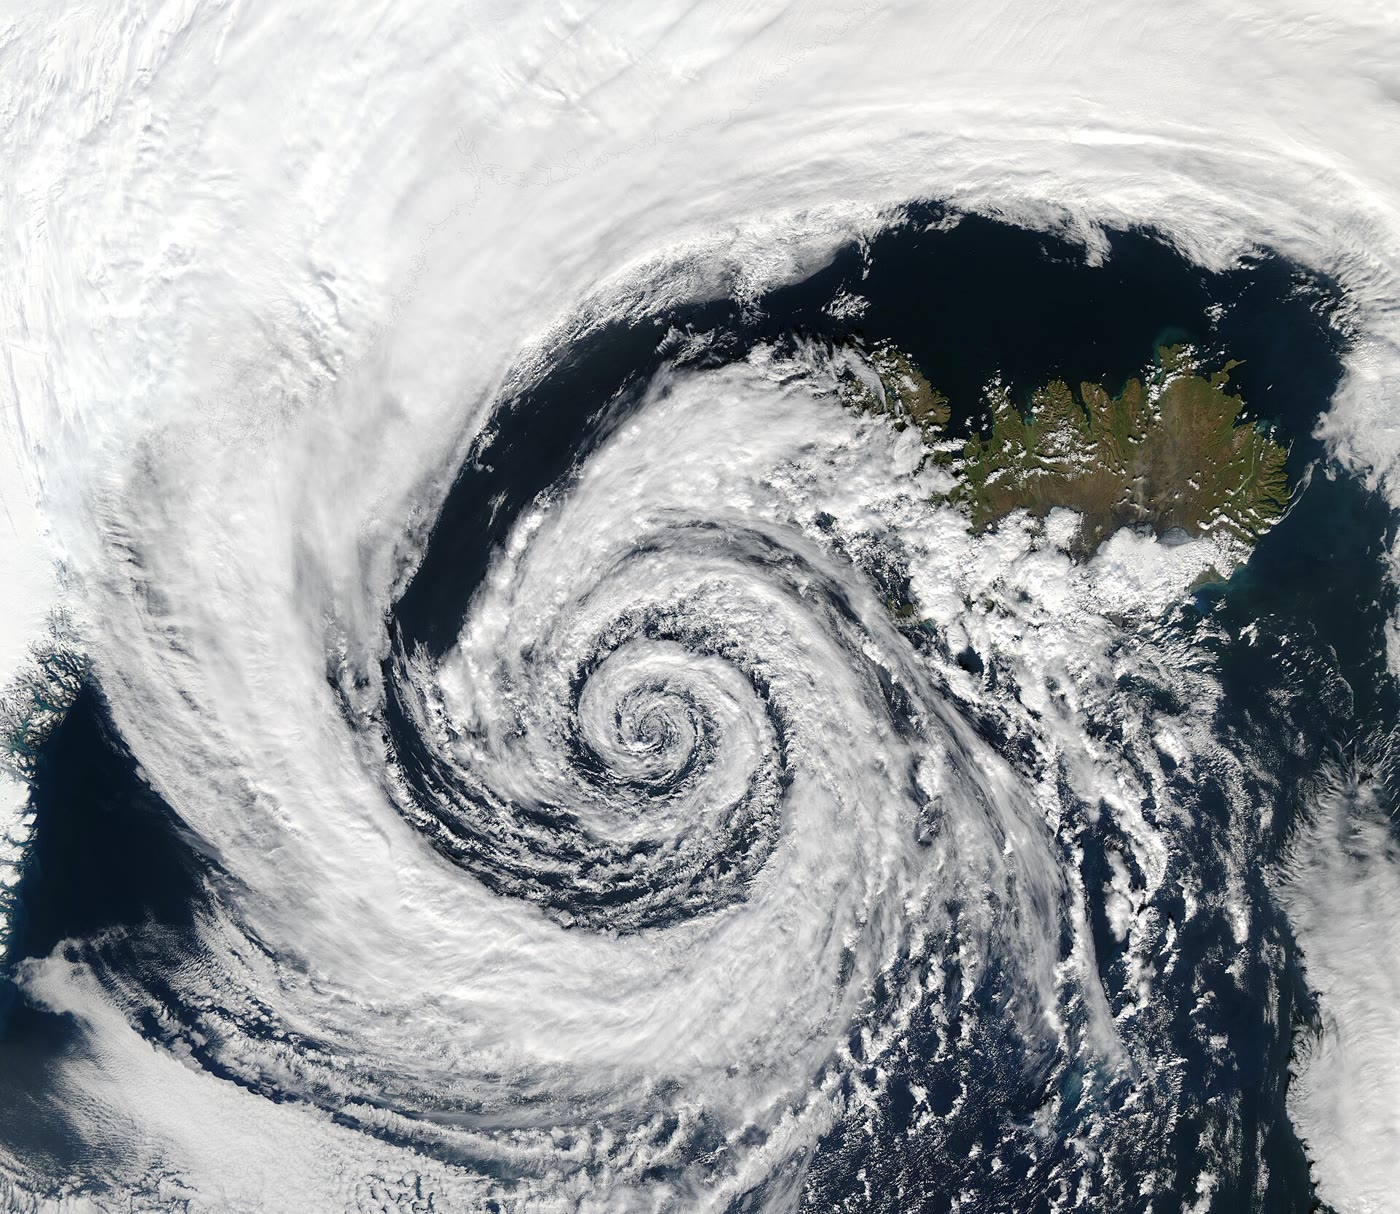
\includegraphics[width=\linewidth]{images/book5/b3-iceland-low.jpg}
\end{minipage}

\par\smallskip{\small 左图：北纬 \ang{45} 一月\omterm{def:b3:atmospheric-dynamics:eddy}{纬向平均}剪切下的伊迪增长率随波长的变化
（NCEP--NCAR Reanalysis~1，
1991--2020），对流层平均层结与 $H = \qty{11}{km}$：
\qty{3200}{km} 以下无增长，增长最快处位于 \qty{4700}{km} 附近。右图：冰岛西南海岸外
一处处于成熟阶段的低压，2003 年 9 月 4 日，其云系
围绕低压中心呈逆时针螺旋状卷曲，
（NASA/GSFC，MODIS Rapid Response Team，公有
领域）。}\label{fig:b3:atmospheric-dynamics:eady}
\end{omfigure}
% ledger: data:b5-ncep-uwnd, nasa:grc-atmos, photo:b3-iceland-low

本科二年级分册中的温带气旋，是正在增长的\omterm{def:b3:gfd-foundations:baroclinic}{斜压}波在地面上的表现：其暖区将暖空气
向极地输送并向上抬升，其后方的冷空气向赤道方向下沉滑移，
高空槽随高度向西倾斜，
这正是\omterm{def:b3:atmospheric-dynamics:ape}{有效位能}释放
所要求的。

\section{大气总环流}\label{sec:b3:atmospheric-dynamics:general-circulation}

大气总环流是通过沿纬圈求平均来描述的，
而平均所略去的部分与其保留的部分同样重要。

\begin{definition}[纬向平均与涡旋]\label{def:b3:atmospheric-dynamics:eddy}
物理量 $A$ 的\emph{纬向平均}\index{纬向平均}，是它在固定高度或固定气压面上
沿纬圈的平均，$[A] =
(1/2\pi)\int_0^{2\pi} A\,\mathrm d\lambda$。偏差 $A^* = A - [A]$
即其涡旋部分；大气中的\emph{涡旋}\index{涡旋}，是指流动
偏离其纬向平均的任何部分，包括行波、
定常波、气旋与反气旋。
\end{definition}

乘积的\omterm{def:b3:atmospheric-dynamics:eddy}{纬向平均}分为两项：$[vT] = [v][T] + [v^*T^*]$。
第一项为平均经向环流的输送，即本科一年级分册中的
环流圈；第二项为\omterm{def:b3:atmospheric-dynamics:eddy}{涡旋}的输送。
在中纬度，平均经向风较弱，\omterm{def:b3:atmospheric-dynamics:eddy}{涡旋}项
占主导：向极运动的空气比同一纬度上向赤道运动的空气更暖，
如下图所示，且 $[v^*T^*] > 0$。\omterm{def:b3:atmospheric-dynamics:eddy}{涡旋}还
将西风动量 $[u^*v^*]$ 从副热带输送到
急流所在的纬度，这正是急流与地面西风带能够
克服摩擦力而得以维持的原因。本科一年级分册中的费雷尔环流圈，是
这种\omterm{def:b3:atmospheric-dynamics:eddy}{涡旋}输送所驱动的平均经向环流。

\begin{omfigure}
\begin{tikzpicture}[>=stealth, font=\small, declare function={s(\x)=0.9*sin(\x r); t(\x)=0.9*sin((\x+1.0) r);}]
\draw[thick, black, domain=0:12.566, samples=120] plot (\x, {s(\x)});
\draw[omThm, thick, densely dashed, domain=0:12.566, samples=120] plot (\x, {t(\x)-0.15});
\foreach \x in {0.3, 6.58} {\draw[->, omThm, very thick] (\x,-1.1) -- (\x,1.15)
  node[above, font=\scriptsize] {暖};}
\foreach \x in {3.45, 9.73} {\draw[->, omDef, very thick] (\x,1.1) -- (\x,-1.15)
  node[below, font=\scriptsize] {冷};}
\node[font=\scriptsize, anchor=west] at (12.7,{s(12.566)}) {流线};
\node[font=\scriptsize, anchor=west, omThm] at (12.7,{t(12.566)-0.15}) {等温线};
\draw[->] (-1.6,-1.1) -- (-0.6,-1.1) node[below, font=\scriptsize] {东};
\draw[->] (-1.6,-1.1) -- (-1.6,-0.1) node[above, font=\scriptsize] {北};
\node[font=\scriptsize] at (6.3,-1.95) {北方为冷空气，南方为暖空气};
\end{tikzpicture}

\par\smallskip{\small 正在增长的\omterm{def:b3:gfd-foundations:baroclinic}{斜压}波的平面图（示意图，
北半球，西风气流）。等温线（虚线）落后于
流线不超过四分之一波长，因此向北运动的空气（红色
箭头）比同一纬度向南运动的空气（蓝色）更暖：
波动将热量向极地输送，$[v^*T^*] >
0$。}\label{fig:b3:atmospheric-dynamics:heatflux}
\end{omfigure}

在热带，\omterm{def:b3:atmospheric-dynamics:eddy}{涡旋}较弱，平均环流将热量向极地输送，
即哈得来环流圈。本科一年级分册指出，离开赤道的空气
若静止并保持其角动量，则在
\ang{40} 处将达到数百米每秒的风速，但未解释
环流圈为何止于 \ang{30} 附近。一个简单模型给出了答案。

\begin{definition}[大气角动量；赫尔德–侯模型]\label{def:b3:atmospheric-dynamics:held-hou}
单位质量的\emph{大气角动量}\index{大气角动量}相对于地球自转轴，
为 $M = (\Omega a\cos\varphi +
u)\,a\cos\varphi$，其中向东风速为 $u$，纬度为 $\varphi$。
哈得来环流圈的\emph{赫尔德–侯模型}\index{赫尔德–侯模型}是一个
轴对称、定常的环流，描述深度为
$H$ 的干 Boussinesq 大气，该大气通过弛豫加热
趋向辐射平衡位温 $\theta_E/\theta_0 = 1 + \Delta/3 - \Delta\sin^2\varphi$；
其上支保持 $M$ 守恒，下支风速可忽略，
且流动满足\omterm{thm:b3:gfd-foundations:thermal-wind}{热成风}平衡。
\end{definition}

\begin{theorem}[哈得来环流圈的范围]\label{thm:b3:atmospheric-dynamics:held-hou}
在小角度极限下，赫尔德–侯环流圈延伸至纬度
\[
\varphi_H = \left(\frac{5\,gH\Delta}{3\,\Omega^2a^2}\right)^{1/2}
\]
在每个半球内，其上支风速为 $u_M = \Omega
a\varphi^2$。
\end{theorem}

\begin{proof}
当 $\varphi$ 很小时，$\cos\varphi \approx 1$，离开赤道时
静止且 $M = \Omega a^2$ 的空气，其 $u_M = \Omega a(1 - \cos^2\varphi)/\cos\varphi
\approx \Omega a\varphi^2$。取 $f \approx 2\Omega\varphi$，$y = a\varphi$，
地面风速为零，\omterm{thm:b3:gfd-foundations:thermal-wind}{热成风}的 Boussinesq 形式在
深度 $H$ 上为 $2\Omega\varphi\,u_M/H = -(g/a\theta_0)\,\partial\theta_M/
\partial\varphi$，其中 $\theta_M$ 为 $\theta$ 在
环流圈内的垂直平均。于是 $\partial(\theta_M/\theta_0)/\partial\varphi = -2\Omega^2a^2
\varphi^3/(gH)$，且 $\theta_M/\theta_0 = A - K\varphi^4$，$K = \Omega^2a^2/
(2gH)$。在环流圈内，环流只输送热量，既不产生也不消耗
热量，因此环流圈的平均温度与辐射平衡相同，即
$\int_0^{\varphi_H}\theta_M\,\mathrm d\varphi = \int_0^{\varphi_H}
\theta_E\,\mathrm d\varphi$。在边界处温度连续：
$\theta_M(\varphi_H) = \theta_E(\varphi_H)$。取 $\theta_E/\theta_0 \approx
B - \Delta\varphi^2$，$B = 1 + \Delta/3$，由第一个条件得 $A - B =
K\varphi_H^4/5 - \Delta\varphi_H^2/3$，由第二个条件得 $A - B = K\varphi_H^4 -
\Delta\varphi_H^2$。相减得 $(4/5)K\varphi_H^4 = (2/3)\Delta
\varphi_H^2$，从而 $\varphi_H^2 = 5\Delta/(6K) = 5gH\Delta/(3\Omega^2a^2)$。
\end{proof}

环流圈止于角动量守恒所要求的温度，
与辐射平衡相遇之处；越过此处，大气就必须
比辐射所使其达到的温度更冷。该模型有两个
不能直接观测的参数。取 $H = \qty{15}{km}$，$\Delta$ 介于 $1/6$ 与
$1/3$ 之间（仅作示例），$\varphi_H$ 为 \ang{25} 至 \ang{35}。
依据\omterm{def:b3:atmospheric-dynamics:eddy}{纬向平均}经向风读得的观测环流圈，年平均情况下止于
北纬 \ang{33.3} 与南纬 \ang{32.5}，冬季较强的环流圈
在 12 月至次年 2 月止于北纬 \ang{30.8}，在
6 月至 8 月止于南纬 \ang{29.1}。关键在于其标度关系：环流圈随对流层加厚
与加热对比增强而变宽，在
自转更快的行星上则变窄。模型的上支风速为 $u_M =
\qty{88}{m/s}$ 位于边界处，取 $\Delta = 1/6$，是观测急流的两倍：
多余部分由\omterm{def:b3:atmospheric-dynamics:eddy}{涡旋}带走。
% ledger: geod5:grs80-defining, earth:Rmean, data:b5-ncep-vwnd (values in figdata/bachelor-3/held_hou.py)

\begin{omfigure}
\begin{tikzpicture}
\begin{groupplot}[group style={group size=2 by 1, horizontal sep=1.7cm},
  width=0.48\linewidth, height=0.44\linewidth, tick label style={font=\scriptsize},
  label style={font=\small}, legend style={font=\scriptsize, draw=none, fill=none}]
\nextgroupplot[xlabel={纬度 (\unit{\degree})}, ylabel={$100\,(\theta/\theta_0 - 1)$},
  xmin=0, xmax=60, ymin=-30, ymax=15, legend pos=south west, legend cell align=left,
  title={\small $\Delta = 1/3$, $H = \qty{15}{km}$}]
% computed in figdata/bachelor-3/held_hou.py
\addplot[omDef, thick] table[x=phi, y=thE] {figdata/out/bachelor-3-held_hou-theta-3.dat};
\addplot[omThm, thick, unbounded coords=jump] table[x=phi, y=thM] {figdata/out/bachelor-3-held_hou-theta-3.dat};
\addplot[black!50, densely dashed, forget plot] coordinates {(35.26,-30) (35.26,15)};
\node[font=\scriptsize, anchor=south west] at (axis cs:35.6,7) {$\varphi_H$};
\legend{$\theta_E$, $\theta_M$}
\nextgroupplot[xlabel={纬度 (\unit{\degree})}, ylabel={$\psi$ 在 \qty{500}{hPa} 处（$10^{10}$\,\unit{kg/s}）},
  xmin=-60, xmax=60, ymin=-25, ymax=25, xtick={-60,-30,0,30,60}, legend pos=south west,
  legend cell align=left]
\addplot[black!50, thin, domain=-60:60, samples=2, forget plot] {0};
\addplot[black, thick] table[x=lat, y=ann] {figdata/out/bachelor-3-held_hou-psi.dat};
\addplot[omDef, thick] table[x=lat, y=djf] {figdata/out/bachelor-3-held_hou-psi.dat};
\addplot[omThm, thick] table[x=lat, y=jja] {figdata/out/bachelor-3-held_hou-psi.dat};
\legend{全年, 12 月至次年 2 月, 6 月至 8 月}
\end{groupplot}
\end{tikzpicture}

\par\smallskip{\small 左图为赫尔德–侯构造：环流圈的角动量守恒温度（红色）
与辐射平衡温度（蓝色）相交于 $\varphi_H = \ang{35}$，环流圈内两曲线
之间的面积相等。右图为 \qty{500}{hPa} 处的平均经向质量流函数，
由\omterm{def:b3:atmospheric-dynamics:eddy}{纬向平均}经向风得出（NCEP--NCAR
再分析~1，1991--2020 年；\qty{500}{hPa} 以上空气向北运动时为正）：
冬半球较强的环流圈
横跨赤道，
各环流圈止于约
\ang{30}。}\label{fig:b3:atmospheric-dynamics:held-hou}
\end{omfigure}
% ledger: data:b5-ncep-vwnd

\begin{history}[从长波到首次数值预报]
1939 年，罗斯贝及其合作者在 \emph{Journal of Marine
Research} 上，力图从单一视角解释天气中若干
看似相互独立的现象。受逆盛行西风向上游移动的天气型启发，
罗斯贝写出了一套线性化理论：大尺度扰动相对于风倾向于向西移动，
小尺度扰动则向东移动。这便是本章的波动
与 $\beta$ 平面。十一年后，查尼、菲约尔托夫特与诺伊曼
在电子计算机 ENIAC 上对\omterm{thm:b3:atmospheric-dynamics:bve}{正压涡度方程}进行了数值积分：
在 \qty{500}{mb} 层面上做了四次 24~小时的预报，
网格距离为 \qty{736}{km}，经度间隔为 8 度，
位于 \ang{45} 纬度处。
每次预报的计算耗时约 24~小时：
正如他们所写，计算速度仅勉强跟得上天气的变化。
\end{history}
% ledger: rossby39:paper, jmr20:commentary, charney50:eniac

\section{练习}

\begin{exercise}[$\star$]\label{exo:b3:atmospheric-dynamics:1}
(a)~求一天转一周的刚体旋转\omterm{def:b3:atmospheric-dynamics:eddy}{涡旋}的\omterm{def:b3:atmospheric-dynamics:vorticity-kinds}{相对涡度}。(b)~求北纬 \ang{30} 与
北纬 \ang{60} 处的\omterm{def:b3:atmospheric-dynamics:vorticity-kinds}{行星涡度}（$\Omega = \qty{7.292e-5}{rad/s}$），
并加以比较。
\end{exercise}

\begin{exercise}[$\star$]\label{exo:b3:atmospheric-dynamics:2}
北纬 \ang{30} 处\omterm{def:b3:atmospheric-dynamics:vorticity-kinds}{相对涡度}为零的气块，
在无辐散的流动中移动至北纬 \ang{40}。求其此处的\omterm{def:b3:atmospheric-dynamics:vorticity-kinds}{相对涡度}，
并判断它是气旋式还是反气旋式的。
\end{exercise}

\begin{exercise}[$\star$]\label{exo:b3:atmospheric-dynamics:3}
在北纬 \ang{45} 处、平均风为零的条件下，求波长为 \qty{5000}{km}、
$l = 0$ 的罗斯贝波的相速，并说明其移动方向。
\end{exercise}

\begin{exercise}[$\star$]\label{exo:b3:atmospheric-dynamics:4}
在北纬 \ang{60} 处、速度为 \qty{10}{m/s} 的西风中，求 $\beta$、
定常波长，以及纬圈上定常波的个数
（$a = \qty{6371}{km}$）。
\end{exercise}

\begin{exercise}[$\star\star$]\label{exo:b3:atmospheric-dynamics:5}
一列厚度为 \qty{10}{km}、在北纬 \ang{45} 处\omterm{def:b3:atmospheric-dynamics:vorticity-kinds}{相对涡度}为零的空气柱，
越过一座山脉时被压缩至 \qty{8}{km}，随后进入厚度为 \qty{12}{km} 的盆地，
假设其始终保持在北纬 \ang{45} 附近，
求其在山脉上空与盆地上空的\omterm{def:b3:atmospheric-dynamics:vorticity-kinds}{相对涡度}。
低压将在何处倾向于形成？
\end{exercise}

\begin{exercise}[$\star\star$]\label{exo:b3:atmospheric-dynamics:6}
对于北纬 \ang{45} 纬圈上有五个波峰、$l = 0$ 的波，
在速度为 \qty{15}{m/s} 的西风中，求其相速与群速度。
该波的能量向东传播 \qty{5000}{km} 需要多长时间，
图样需要多长时间？
\end{exercise}

\begin{exercise}[$\star\star$]\label{exo:b3:atmospheric-dynamics:7}
在北纬 \ang{45} 处、速度为 \qty{15}{m/s} 的西风中，一列波被限制在若干纬度之间，
使得 $l = \pi/(\qty{6000}{km})$。(a)~求其定常纬向波数与波长。
(b)~证明对于
$l = \pi/(\qty{3000}{km})$，不存在定常波。
\end{exercise}

\begin{exercise}[$\star\star$]\label{exo:b3:atmospheric-dynamics:8}
在北纬 \ang{45} 处的\omterm{def:b3:atmospheric-dynamics:eady}{伊迪模型}中，$\Lambda = \qty{2e-3}{s^{-1}}$，$N =
\qty{0.012}{s^{-1}}$，$H = \qty{10}{km}$。求 $L_d$、增长最快扰动的增长率
与 $e$ 折时间，以及该扰动的
波长。
\end{exercise}

\begin{exercise}[$\star\star$]\label{exo:b3:atmospheric-dynamics:9}
沿纬圈，\omterm{def:b3:atmospheric-dynamics:eddy}{涡旋}经向风为 $v^* = V\cos kx$，\omterm{def:b3:atmospheric-dynamics:eddy}{涡旋}温度为
$T^* = T_0\cos(kx - \delta)$，其中 $V = \qty{10}{m/s}$ 与
$T_0 = \qty{5}{K}$。求 $[v^*T^*]$ 在 $\delta = 0$、\ang{60} 与
\ang{90} 时的值，以及对应的热流量 $\rho c_p[v^*T^*]$
每 \unit{kg/m^3} 空气（$c_p = \qty{1004}{J.kg^{-1}.K^{-1}}$）。哪一种
排列不输运热量？
\end{exercise}

\begin{exercise}[$\star\star\star$]\label{exo:b3:atmospheric-dynamics:10}
从\omterm{thm:b3:atmospheric-dynamics:bve}{正压涡度方程}出发，
推导均匀西风中罗斯贝波的色散关系，并证明相对于
空气，每一个罗斯贝波都向西运动。
\end{exercise}

\begin{exercise}[$\star\star\star$]\label{exo:b3:atmospheric-dynamics:11}
在\omterm{def:b3:atmospheric-dynamics:held-hou}{赫尔德–侯模型}中取 $H = \qty{12}{km}$，$\Delta = 1/4$，计算
$\varphi_H$、边缘处的小角度风 $u_M$ 以及
该处的精确角动量风，并与一月\omterm{def:b3:atmospheric-dynamics:eddy}{纬向平均}中的副热带急流
（\qty{44}{m/s}）进行比较。
\end{exercise}

\begin{exercise}[$\star\star\star$]\label{exo:b3:atmospheric-dynamics:12}
两层空气在 \qty{300}{K} 时位温相差 \qty{10}{K}；其界面
沿极地方向以斜率 $s$ 向上倾斜，
跨越宽 \qty{4000}{km} 的纬向带，且 $\rho = \qty{0.7}{kg/m^3}$。(a)~证明界面趋于平坦时，
单位面积释放的能量为 $\rho g' s^2L^2/24$，
其中 $g' = g\,\Delta\theta/\theta$。(b)~计算 $s = 10^{-3}$ 与
$2\times10^{-3}$ 时的该能量，并与同一空气中风速为 \qty{15}{m/s} 的
风穿过 \qty{10}{km} 厚气层的动能进行比较。
\end{exercise}
% ledger: geod5:grs80-defining, earth:Rmean, data:b5-ncep-uwnd

\section{问题：静止的波}

\begin{problem}[{周末问题——涡度、罗斯贝波与北纬 \ang{45} 处
\omterm{def:b3:gfd-foundations:baroclinic}{斜压}波的增长}]
\label{pb:b3:atmospheric-dynamics:1}
一股 \qty{15}{m/s} 的西风穿过一块虚构大陆的中纬度地区，
沿北纬 \ang{45} 方向。取 $\Omega =
\qty{7.292115e-5}{rad/s}$，$a = \qty{6371}{km}$ 与 $g = \qty{9.81}{m/s^2}$。
该气流的所有数值均为虚构。

\medskip\noindent\textbf{第一部分——偏移的气块。}
\begin{enumerate}
\item 北纬 \ang{45} 处无\omterm{def:b3:atmospheric-dynamics:vorticity-kinds}{相对涡度}的气块被推向
  北纬 \ang{50}。计算两个纬度处的 $f$，以及北纬 \ang{50} 处的\omterm{def:b3:atmospheric-dynamics:vorticity-kinds}{相对涡度}，
  若气流无散度。
\item 以 \qty{15}{m/s} 运动，沿多大的曲率半径转弯
  （取 $\zeta = -V/R$，全部来自曲率）？向哪一侧转弯？
\item 若其气柱在途中也从 \qty{10.0}{km} 压缩至 \qty{9.5}{km}，
  则北纬 \ang{50} 处的\omterm{def:b3:atmospheric-dynamics:vorticity-kinds}{相对涡度}为多少？
\item 若改将气块推向北纬 \ang{40}，且无散度，
  其获得的\omterm{def:b3:atmospheric-dynamics:vorticity-kinds}{相对涡度}为多少？解释为何偏离
  其纬度的气块会绕该纬度振荡。
\end{enumerate}

\medskip\noindent\textbf{第二部分——行波。}
\begin{enumerate}[resume]
\item 计算北纬 \ang{45} 处的 $\beta$ 以及该纬圈的长度。
\item 对沿纬圈的 $n = 3$ 至 8 个波（$l = 0$），计算
  其波长、相速与群速度，
  均在 \qty{15}{m/s} 的西风中求取。
\item 哪些波向西运动，哪些向东运动？波
  $n = 5$ 移动 \qty{1000}{km} 需要多少天？
\item 大陆西部上空的一个脊增强。
  波 $n = 6$ 的影响将在何处、经过多长时间，
  传到下游 \qty{5000}{km} 处？
\end{enumerate}

\medskip\noindent\textbf{第三部分——静止的波。}
\begin{enumerate}[resume]
\item 计算北纬 \ang{45} 处的\omterm{prop:b3:atmospheric-dynamics:stationary}{定常罗斯贝波长}与
  定常波数。
\item 计算西风为 10 与
  \qty{20}{m/s} 时的定常波数。冬季西风增强时，定常波
  会发生什么变化？
\item 计算北纬 \ang{35} 与北纬 \ang{55} 处的定常波数，
  取 \qty{15}{m/s} 的西风。
\item 大陆西部的山脉升高 \qty{2}{km}，伸入深 \qty{10}{km} 的对流层。
  计算一个不改变纬度而穿越这些山脉的气柱的\omterm{def:b3:atmospheric-dynamics:vorticity-kinds}{相对涡度}。
  为何山脉会激发
  定常波？
\item 为何山脉激发的波型只有在
  其波长接近 $\lambda_s$ 时才会静止不动？
\end{enumerate}

\medskip\noindent\textbf{第四部分——风暴的增长。}
\begin{enumerate}[resume]
\item 西风自地面到 \qty{10}{km} 高处增加了
  \qty{25}{m/s}。计算切变 $\Lambda$，以及在平均温度为
  \qty{250}{K} 时，\omterm{thm:b3:gfd-foundations:thermal-wind}{热成风}所隐含的
  极向温度梯度。
\item 取 $N = \qty{0.011}{s^{-1}}$，计算理查森数
  $N^2/\Lambda^2$。该气流是否会对小尺度切变湍流失稳？
\item 计算罗斯贝半径 $L_d$，取 $H = \qty{10}{km}$。
\item 计算增长最快的伊迪扰动的波长，以及
  绕纬圈的此类波的数目。
\item 计算能够增长的最短波长。
\item 计算增长率 $\sigma_{\max}$。
\item 扰动在三天内增长为原来的多少倍？
\item 比较增长中风暴的波长与第三部分的\omterm{prop:b3:atmospheric-dynamics:stationary}{定常罗斯贝波长}，
  哪一个更长？这对风暴相对于定常波的
  运动意味着什么？
\item 增长波的槽随高度向哪一侧倾斜，
  以及为何必须如此？
\item 给出增长最快的伊迪扰动的 $e$ 折时间。
\end{enumerate}
\end{problem}
% ledger: geod5:grs80-defining, earth:Rmean
